\section{Metodología}
\label{cap-metodo}

\subsection{Recolección de datos}
Este paso consistió en grabar vídeos en entornos urbanos con el lente de un dispositivo celular. Estas grabaciones se realizaron a 1080p/30 FPS, idealmente bajo condiciones lumínicas naturales y con el objetivo de que un solo individuo, por grabación, se mueva al rededor de diferentes distancias conocidas en las que pueda ser identificado en dicho video.

El dispositivo de grabación fue un teléfono celular Google Pixel 6 Pro, a través de su cámara principal en la que el sensor está compuesto por 50 millones de píxeles, cada píxel del sensor tiene un tamaño de 1.2 micrómetros y en total el sensor de imagen tiene un tamaño de 1/1.31 pulgadas. Esta cámara permite un campo de visión de 82 grados \cite{Google}.

La grabación se realizó con la perspectiva de la cámara fija, en tal perspectiva se colocó el dispositivo celular en forma horizontal a una altura de 150 centímetros y en un ángulo parcialmente fijo, el individuo se desplazó a lo largo de las distancias conocidas marcadas previamente con un flexómetro procurando caminar al rededor de ellas para cubrir cierta cantidad de frames con cada una de las distancias de interés (Ver Fig.\ref{fig:diag_fija}).

\begin{figure}
    \centering
    \includegraphics[width=1\linewidth]{images/metodologia/diagrama_fija.png}
    \caption{Grabación con cámara fija}
    \label{fig:diag_fija}
\end{figure}

La grabación se realizó con diez voluntarios, cada uno con sus respectivas alturas (Figura \ref{fig:datos_alturas}), medidas previamente a su participación; se buscó mantener alturas variadas, con el fin de evitar el sesgo de la altura más común que es de 1.70 m \cite{Velez_2025}  y que el primer subconjunto de datos presentaba.

\subsection{Generación del conjunto de datos}

\begin{figure}
    \centering
    \includegraphics[width=\linewidth]{images/metodologia/prepro_diag.pdf}
    \caption{Pasos para etiquetar los videos y obtener anotaciones en CSV}
    \label{fig:diag_etiquetado}
\end{figure}

Este proceso consta de cuatro pasos principales (ver Fig.\ref{fig:diag_etiquetado}), los cuales permiten obtener tanto los frames etiquetados con la presencia de un cuadro envolvente en la persona de interés, así como, las anotaciones relevantes en un archivo CSV.

En primer lugar el video se subdivide en los frames correspondientes, a través de OpenCV, debido a que es importante mantener la cantidad de píxeles originales para hacer el cálculo de la distancia no se redimensiona la imagen, por lo tanto, cada frame se procesa con un tamaño de 1080x1920 pixeles.

A continuación se pasa cada frame por el algoritmo de DeepSORT que utiliza YOLOv8, con el objetivo de detectar a personas en el video, identificar quién de ellas es el objetivo principal, aprender características de ésta persona en particular y poder seguirla a lo largo de toda la trayectoria que ésta tomará en el transcurso de grabación.

Lo anterior permite generar un cuadro envolvente de la misma persona en cada frame, y con ello las coordenadas que lo conforman. Posteriormente se aplica la condición de muestre, ya que muchos de los frames son muy parecidos y aportan poca información. Ésta consiste en verificar si ya han pasado 5 frames anteriormente o si por medio del cálculo de la intersección sobre la unión (IOU por sus siglas en inglés) se determina que los frames no son parecidos; cualquiera de estas dos situaciones permite que el frame siga procesándose, en caso contrario se omite y se pasa al frame siguiente.

Con la información proporcionada por el cuadro envolvente se calcula la altura de la persona en píxeles que junto con las características de la cámara y la altura real de la persona en milímetros se realiza la estimación de la distancia con el modelo matemático (\ref{eq:distancia}) usado en \cite{wu2018sizetodepthnewperspectivesingle}.

\begin{equation}
    \text{distancia} = \frac{\text{altura}_{\text{real}}[\text{mm}] \cdot \text{distancia}_{\text{focal}}[\text{mm}] \cdot \text{tamaño}_{\text{sensor}}[\text{px}]}{\text{altura}_{\text{frame}}[\text{px}] \cdot \text{tamaño}_{\text{sensor}}[\text{mm}]}
    \label{eq:distancia}
\end{equation}

Finalmente se guardan los frames etiquetados, cada uno con su identificador de video y de persona, así como las anotaciones de: coordenadas del cuadro envolvente, coordenadas de su punto central, altura, ancho y distancia estimada para todos los videos en un único archivo CSV.
\subsection{Preprocesamiento de datos}
\begin{figure}
    \centering
    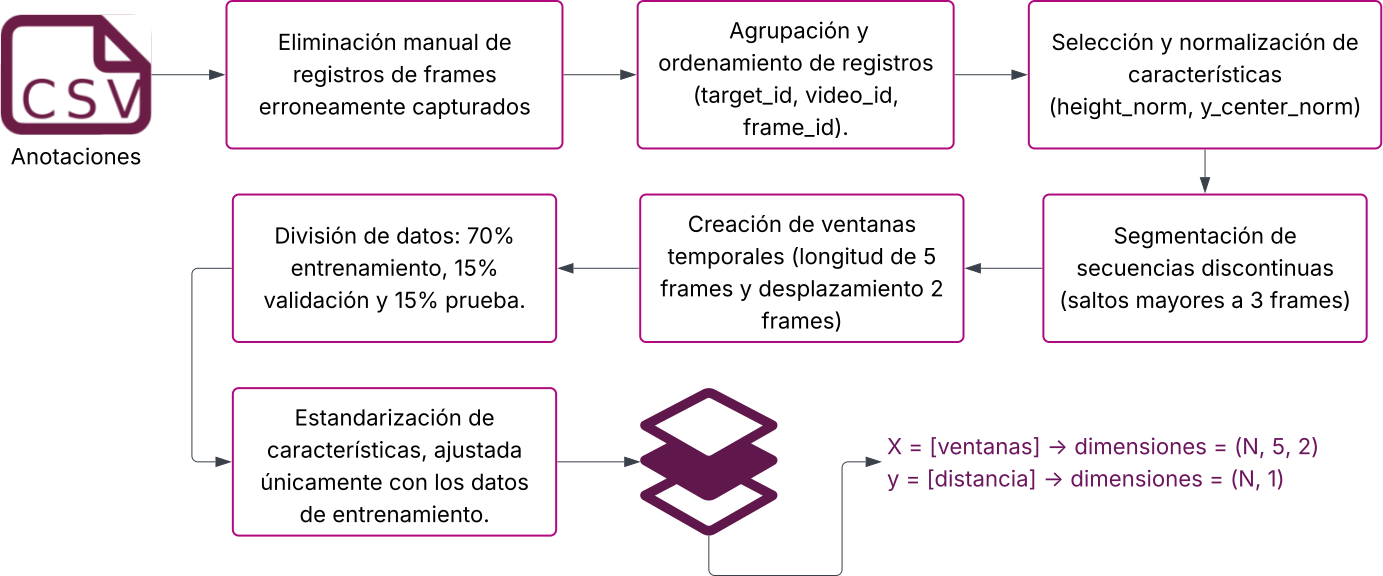
\includegraphics[width=\linewidth]{images/metodologia/preprocess_data.pdf}
    \caption{Preprocesamiento de los datos}
    \label{fig:diag_preprocess}
\end{figure}

El preprocesamiento de los datos está compuesto por ocho pasos fundamentales (ver Fig. \ref{fig:diag_preprocess}). En primer lugar se observó que algunas anotaciones con respecto a la distancia real, proporcionada por el modelo de la Eq.\ref{eq:distancia}, estaban incorrectas; lo anterior debido a que la detección de la persona por medio de DeepSORT (ver Fig.\ref{fig:diag_etiquetado}) fue errónea. Algunos casos debido al cambio de la persona de interés por otra diferente que entraba en el campo de visión, así como, por objetos que eran detectados como la persona de interés tras movimiento determinados del individuo grabado. Lo anterior provocaba que las variables utilizadas por la Eq.\ref{eq:distancia} fueran incorrectas y, por lo tanto, las distancias anotadas también lo fueran. De tal manera que se determinó eliminar de forma manual las anotaciones que se detectaron con esas incongruencias.

A continuación, debido a la naturaleza secuencial de las redes recurrentes, se realizó la agrupación de los datos por medio del identificador de la persona y del video, esto con el fin de evitar que el modelo fuera entrenado con una secuencia que saltara de una persona a otra. 

El paso siguiente fue la selección de las características, con base en los datos proporcionados, las características relevantes tomadas fueron: la coordenada vertical del punto central del recuadro envolvente y la altura de éste recuadro. La normalización consistió en dividir dichos valores entre 1080 (altura en pixeles del frame); de tal forma que se pasa de tener las características en pixeles a tenerlas en valores de 0 a 1. 

Debido a la previa eliminación de frames con datos erróneos, la secuencia de imágenes pudo haber perdido su consistencia temporal, para corregir esto se realizaron segmentaciones; lo anterior consiste en verificar si la secuencia perdió más de 3 frames durante la limpieza de datos, y de ser así se divide la secuencia en dos diferentes, con el punto de corte justo en la posición de la pérdida de frames. Al finalizar este proceso se obtienen múltiples cadenas de frames con una correcta consistencia temporal.

Las redes neuronales recurrentes reciben secuencias de información para predecir el valor final; por lo tanto, se utiliza un tamaño de ventana que define cuántos valores va a recibir la red por cada muestra. El tamaño de ventana propuesto es de cinco valores, de cada secuencia original se tomarán esos cinco valores y se seleccionarán con un desplazamiento de dos frames hacia adelante. Además, lo anterior permite aumentar el numero de muestras, de acuerdo a la Eq.\ref{eq:n_ventanas} y mantener la dinámica temporal de la secuencia.

\begin{equation}
    N_{\text{ventanas}} = \left\lfloor \frac{L - \text{longitud\_ventana}}{\text{desplazamiento}} \right\rfloor + 1
    \label{eq:n_ventanas}
\end{equation}

Finalmente se realizó la división del conjunto de entrenamiento en un 70 porciento y 15 porciento tanto para validación como para prueba. Dentro del conjunto de entrenamiento se forzó a que los datos del individuo con la menor altura (1.51) estuvieran presentes. Con los datos de entrenamiento se ajustó la estandarización de características y se aplicaron a los demás subconjuntos.
Cada muestra tiene una dimensión de (5,2), correspondiente a 5 frames y dos características cada uno, por otro lado, el objetivo (\textit{target}) es la distancia correspondiente al último \textit{frame} en milímetros.

\subsection{Modelo de red neuronal recurrente híbrida}
\begin{figure}
    \centering
    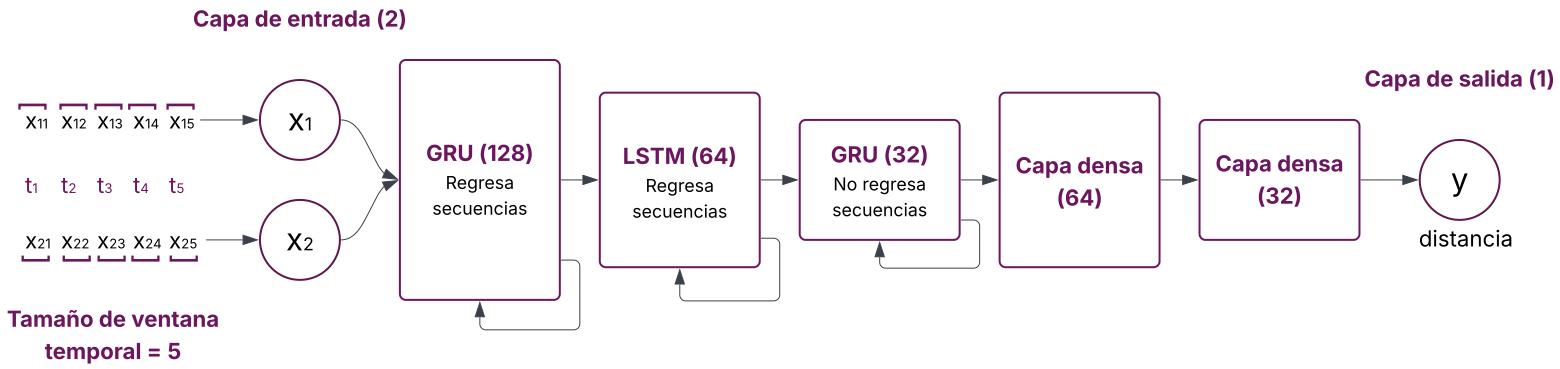
\includegraphics[width=\linewidth]{images/metodologia/nn_diagram.pdf}
    \caption{Arquitectura de la RNN híbrida}
    \label{fig:diag_nn}
\end{figure}

Debido a la naturaleza secuencial de los datos, se propone una arquitectura de red con capas de LSTM y GRU (ver Fig.\ref{fig:diag_nn}). Se tiene una entrada temporal de dos variables seguida de dos capas recurrentes y dos densas con una salida de una sola unidad. Las capas recurrentes utilizan la función de activación \texttt{tanh} para las activaciones principales y \texttt{sigmoid} para las demás, mientras que en las capas intermedias densas se utiliza \texttt{ReLU} y en la capa de salida la función \texttt{lineal}.

La función de pérdida utilizada es el error cuadrático medio (\texttt{MSE}) con el optimizador \texttt{Adam}; adicionalmente se monitorea también el error absoluto medio \texttt{MAE}. Con respecto a la regularización, se aplica \texttt{L2} de $5 \times 10^{-5}$  en las primeras dos capas recurrentes y de $1 \times 10^{-4}$ en las capas densas; se aplica \texttt{dropout} de $0.15$ para las primeras dos capas recurrentes y para las capas densas $0.25$ y $0.15$ respectivamente; también se implementaron mecanismos de regularización adaptativa mediante \texttt{EarlyStopping} y \texttt{ReduceLROnPlateau} de Keras. Las métricas de evaluación registradas son \texttt{MAE}, \texttt{MSE}, \texttt{RMSE}, \texttt{$R^{2}$}, \texttt{MAPE} y \texttt{$\sigma(AE)$}.